\section*{Задание 1: Описание и структурный анализ программного кода}
\subsection{Постановка задачи}
\noindent
Язык: C\# \\
Алгоритм: Генератор лабиринта (DFS + Backtracking) \\
Специфика кода: Рекурсия, двумерные массивы, битовые маски стен, однобуквенные переменные, магические числа \\
Контекст: Генерация процедурных карт для симуляции перемещения роботов\\
\vspace{0.5em}
Необходимо:
\begin{enumerate}
\item Сгенерировать «грязный» (нечитаемый, обфусцированный) код указанного алгоритма.
\item Провести его анализ: определить назначение, расшифровать переменные, визуализировать логику, проверить гипотетические сценарии.
\item Синтезировать итоговую структурированную документацию.
\end{enumerate}

\subsection{Гипотеза и системный промпт (этап 0 – генерация «грязного» кода)}
Промпт (основной модели):
\textit{«Ты – небрежный разработчик, который пишет рабочий, но максимально нечитаемый код на C\#. Реализуй генератор лабиринта с использованием алгоритма поиска в глубину (DFS) и backtracking. Функция должна принимать ширину и высоту лабиринта и возвращать двумерный массив целых чисел. Используй только стандартные типы, без внешних библиотек. Замени все осмысленные имена переменных на однобуквенные (g, r, c, k, m, d, b). Удали все комментарии, XML-doc и директивы using. Используй магические числа для направлений и состояний стен. Применяй битовые маски (сдвиги <<, операторы \& и |) для кодирования стен в ячейках. Сверни вычисления в сложные однострочные конструкции где возможно. Код должен компилироваться и работать логически верно.»}\\
\vspace{0.5em}
Ответ модели:
\newpage
\lstinputlisting{z1/0.cs}
\noindent
\indent Анализ: Код синтаксически корректен, но использует абстрактные имена переменных, повсеместно применены рекурсивные вызовы без явной проверки глубины, битовые маски (1, 2, 4, 8) жестко закодированы. Отсутствует валидация входных размеров. Логика backtracking скрыта в условных переходах.

\subsection{Журнал диалога и итераций (работа с основной моделью)}
\noindent
\textbf{Этап 1. Первичный контекстный анализ (Zero-shot Scoping)} \\
\indent Промпт:
\textit{«Ты – Senior C\# Developer, проводящий технический аудит legacy-кода. Посмотри на этот код. Не вдаваясь в детали реализации, определи общее назначение программы, какие входные данные она ожидает и какой результат выдаёт. Назови возможную предметную область.»}\\
\vspace{0.5em}
Ответ модели:
\begin{figure}[H]
\centering
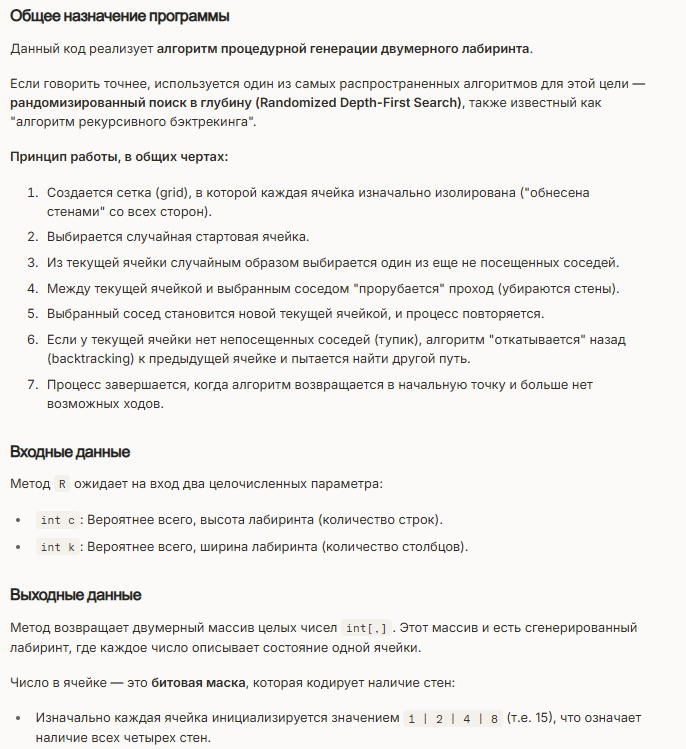
\includegraphics[width=16cm]{z1/1-1.png}
\caption{ч.1}
\end{figure}
\vspace{0.5em}
\begin{figure}[H]
\centering
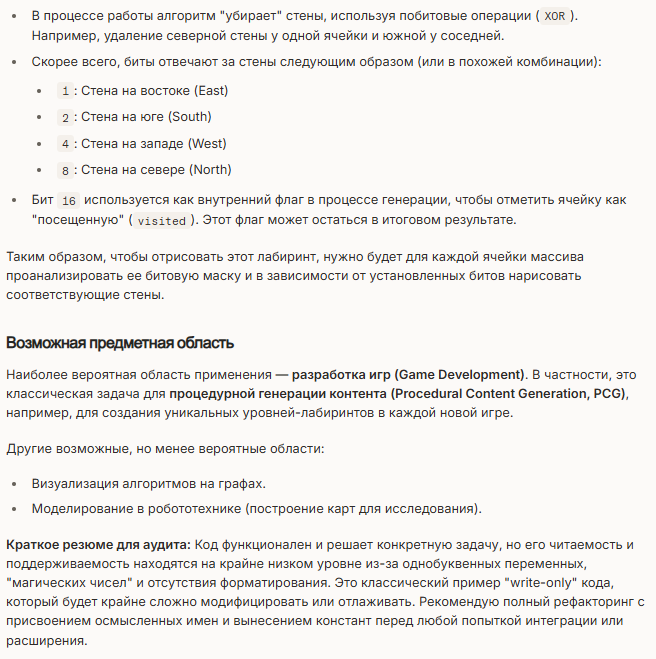
\includegraphics[width=16cm]{z1/1-2.png}
\caption{ч.2}
\end{figure}
\noindent
\indent Анализ: Модель корректно идентифицировала алгоритм процедурной генерации лабиринта на основе DFS. Указаны входные параметры (размеры сетки) и выходные данные (массив состояний ячеек). Предметная область определена верно (симуляция, игровые движки, робототехника). Корректировка не потребовалась.

\vspace{0.5em}
\noindent
\textbf{Этап 2. Глубокая интерпретация и деобфускация переменных} \\
\indent Промпт (с применением Chain of Density):
\textit{«Проведи построчный анализ. Для каждой переменной объясни её функциональную роль в контексте DFS и backtracking. Почему используется рекурсия? Что означают магические числа 1, 2, 4, 8? Как работают побитовые операции в контексте хранения стен? Выдай ответ в виде таблицы.»}\\
\vspace{0.5em}
Ответ модели:
\begin{figure}[H]
\centering
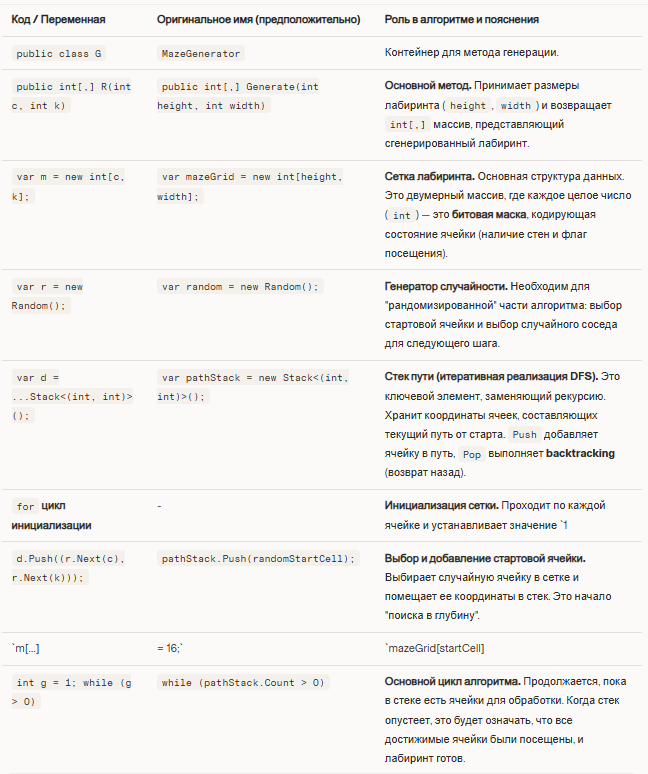
\includegraphics[width=15cm]{z1/2-1.png}
\caption{ч.1}
\end{figure}
\vspace{0.5em}
\begin{figure}[H]
\centering
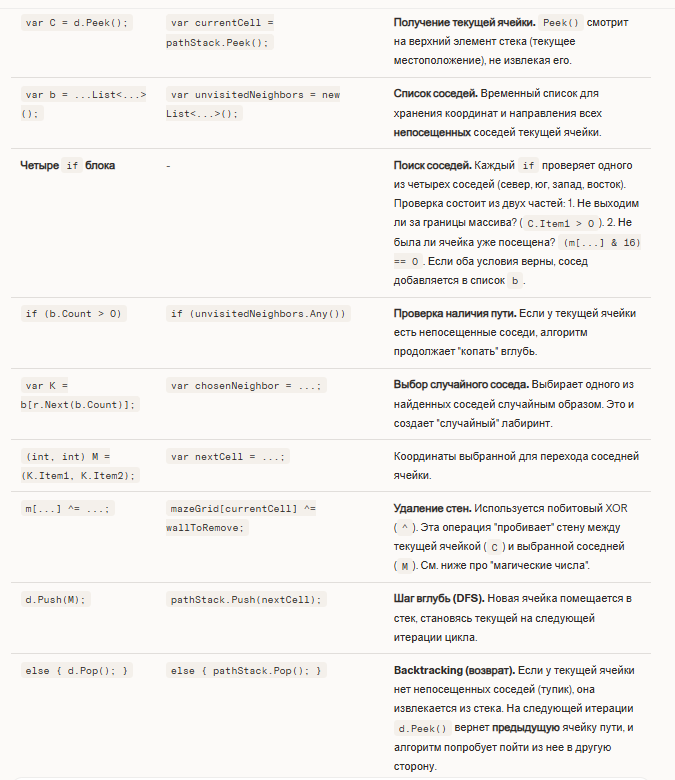
\includegraphics[width=16cm]{z1/2-2.png}
\caption{ч.2}
\end{figure}
\noindent
\indent Анализ: Ответ детализирован, но таблица была частично разбита текстом. \\
\vspace{0.5em}
\indent Корректирующий промпт:
\textit{«Отлично. Теперь представь расшифровку переменных строго в виде таблицы: старое имя → осмысленное имя (например, r → row) и краткое техническое описание. В ответ выдай только таблицу.»}\\
\vspace{0.5em}
Ответ модели:
\begin{figure}[H]
\centering
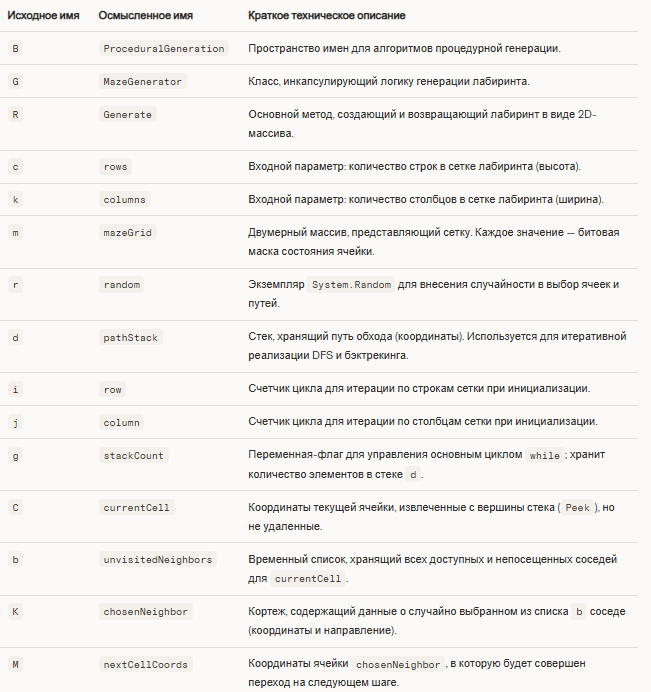
\includegraphics[width=17cm]{z1/3-1.png}
\caption{Таблица деобфускации}
\end{figure}

\vspace{0.5em}
\noindent
\textbf{Этап 3. Структурная абстракция и визуализация логики} \\
\indent Промпт:
\textit{«Сгенерируй псевдокод этого алгоритма на русском языке, опустив синтаксический шум C\#. Затем создай описание блок-схемы в формате Mermaid (код, который можно вставить в Markdown).»}\\
\vspace{0.5em}
\noindent
Ответ модели (псевдокод): \\
\begin{figure}[H]
\centering
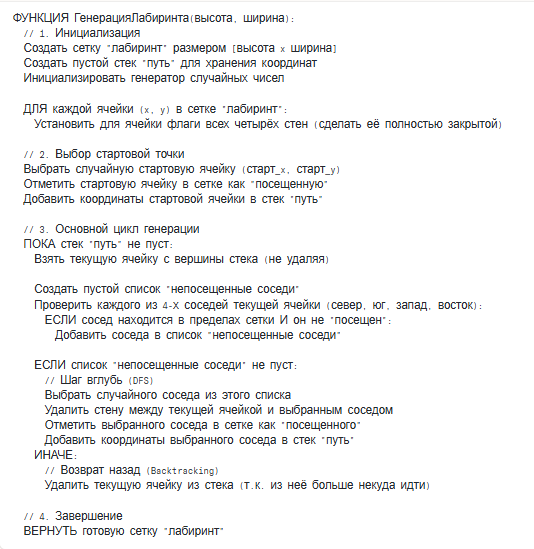
\includegraphics[width=16cm]{z1/4-1.png}
\caption{Псевдокод на русском}
\end{figure}
\vspace{0.5em}
Блок-схема в формате Mermaid:
\begin{figure}[H]
\centering
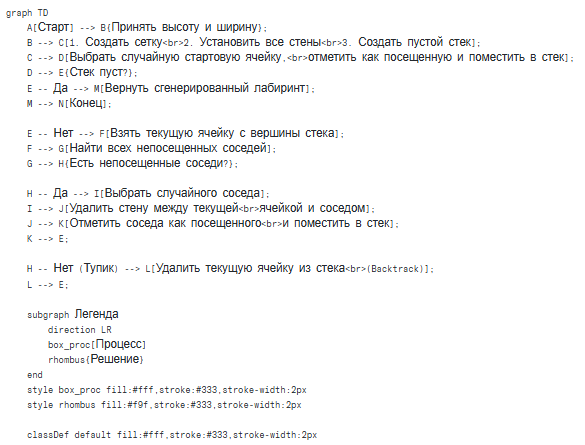
\includegraphics[width=16cm]{z1/4-2.png}
\caption{Блок-схема алгоритма}
\end{figure}
Анализ: Псевдокод точно отражает рекурсивную природу и механизм backtracking. Mermaid-диаграмма корректно визуализирует ветвление и условия возврата.

\vspace{0.5em}
\noindent
\textbf{Этап 4. Верификация через гипотетическое тестирование (Socratic Method)} \\
Промпт:
\textit{«Ответь на вопросы, ссылаясь на конкретные строки исходного кода:
1. Что произойдёт, если на вход подать отрицательные или нулевые размеры (w <= 0 или h <= 0)?
2. Как поведёт себя код при генерации лабиринта 10000x10000?
3. Есть ли в коде потенциальная неэффективность или риск StackOverflowException?»} \\
\vspace{0.5em}
Ответ модели:
\begin{figure}[H]
\centering
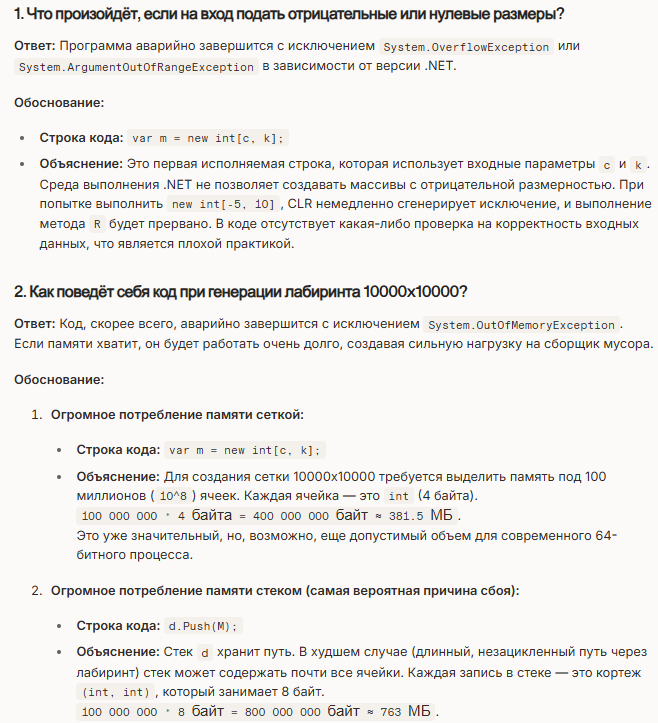
\includegraphics[width=15cm]{z1/5-1.png}
\caption{ч.1}
\end{figure}
\vspace{0.5em}
\begin{figure}[H]
\centering
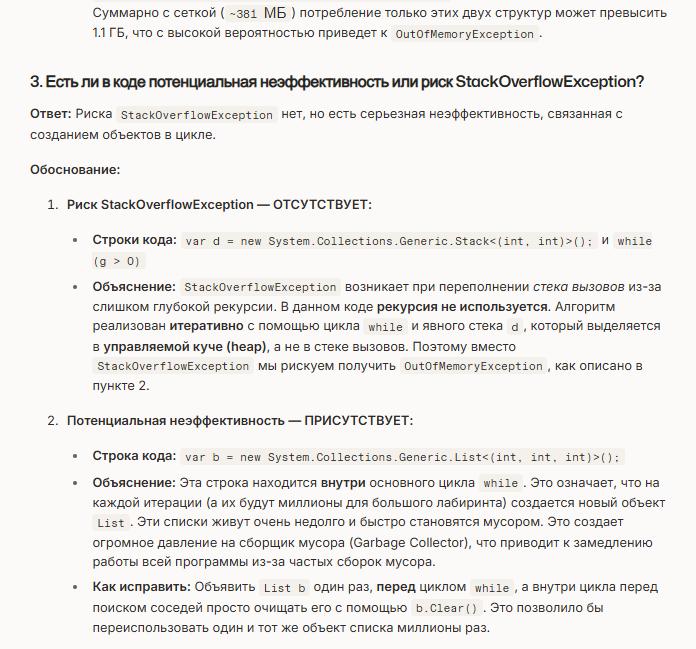
\includegraphics[width=16cm]{z1/5-2.png}
\caption{ч.2}
\end{figure}
Анализ: Модель точно симулировала выполнение: указала на отсутствие валидации входных данных (возникнет IndexOutOfRangeException), выявила критический риск переполнения стека при больших размерах из-за глубокой рекурсии, отметила отсутствие явного управления памятью (GC справится, но задержки возможны). Корректировка не потребовалась.

\vspace{0.5em}
\noindent
\textbf{Этап 5. Синтез итоговой документации} \\
\indent Промпт:
\textit{«Объедини всю информацию из диалога в единый структурированный документ, который включает:
Исходный «плохой» код,
Краткое резюме назначения,
Таблицу расшифровки переменных,
Пошаговое описание алгоритма на русском,
Выявленные ограничения и потенциальные проблемы.
Документ должен выглядеть как профессиональная документация.»} \\
\vspace{0.5em}
\noindent
Модель выдала итоговый документ (см. раздел 1.4).

\subsection{Артефакты}
Исходный «грязный» код:
\lstinputlisting{z1/0.cs}
\vspace{0.5em}
Итоговое структурированное описание алгоритма от модели:
\begin{figure}[H]
\centering
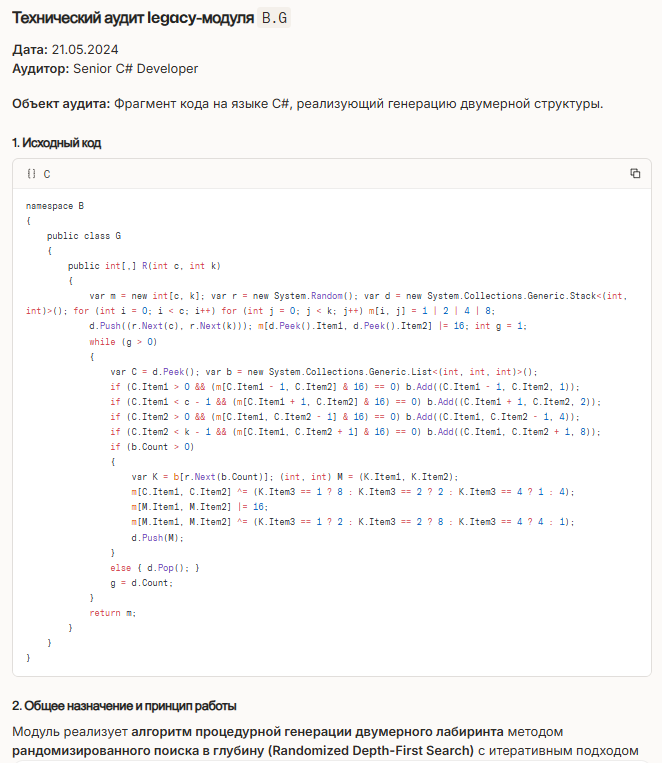
\includegraphics[width=17cm]{z1/6-1.png}
\caption{ч.1}
\end{figure}
\vspace{0.5em}
\begin{figure}[H]
\centering
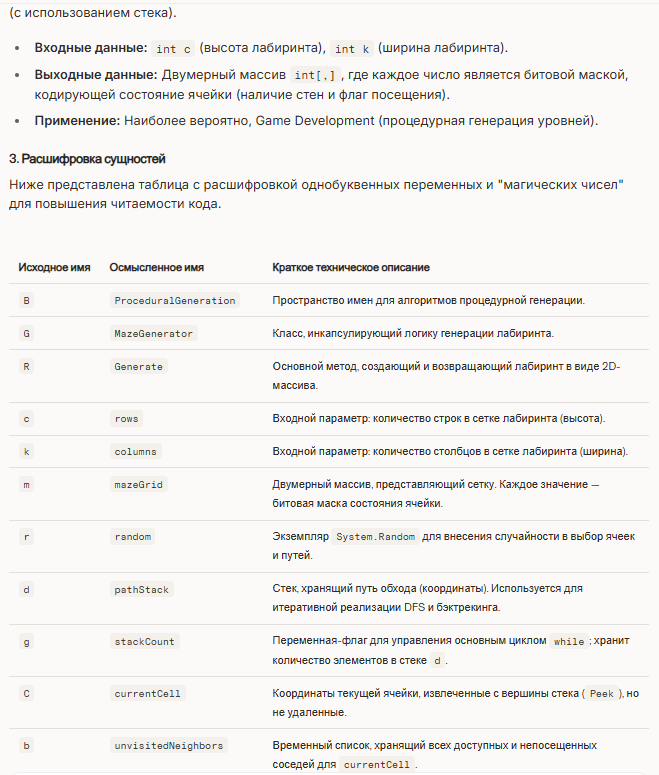
\includegraphics[width=17cm]{z1/6-2.png}
\caption{ч.2}
\end{figure}
\vspace{0.5em}
\begin{figure}[H]
\centering
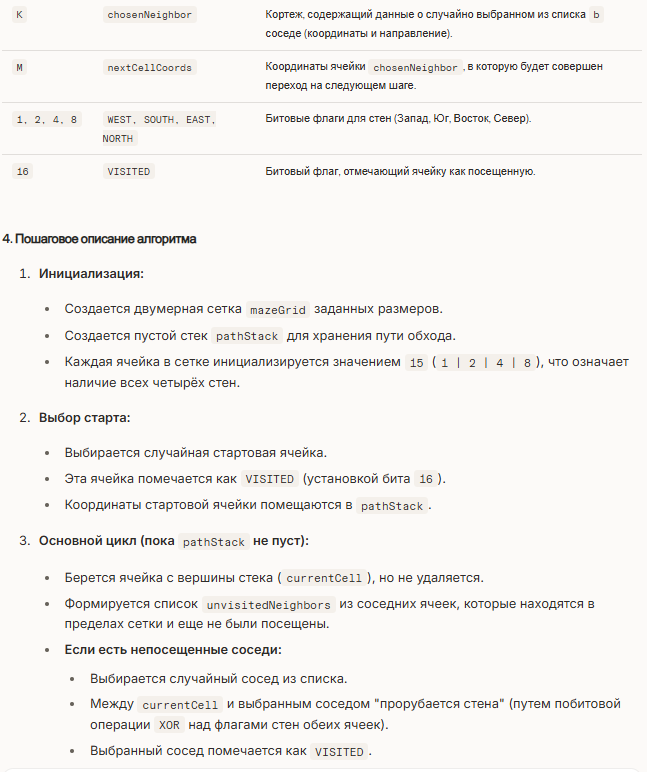
\includegraphics[width=17cm]{z1/6-3.png}
\caption{ч.3}
\end{figure}
\centering
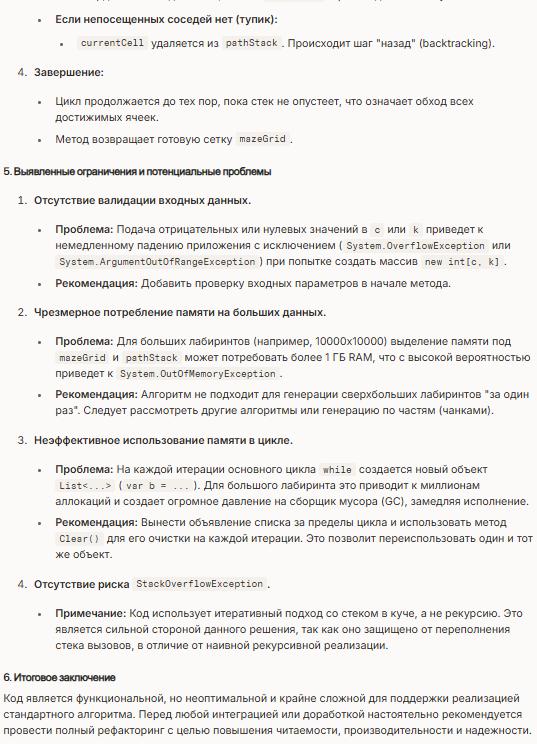
\includegraphics[width=17cm]{z1/6-4.png}
\caption{ч. 4}
\end{figure}

\subsection{Сравнение моделей (Benchmarking)}
\begin{table}[h!]
\centering
\begin{tabular}{|l|p{5cm}|p{5cm}|}
\hline
\textbf{Критерий} & \textbf{модель (a)} & \textbf{модель (b)} \\
\hline
Глубина деобфускации & 5 & 4 \\
\hline
Полнота описания алгоритма & 4 & 5 \\
\hline
Корректность визуализации Mermaid & 5 & 3 \\
\hline
Способность к самокоррекции & 4 & 5 \\
\hline
\textbf{Итог} & 4.5 & 4.25\\
\hline
\end{tabular}
\end{table} \\
Итог: Обе модели успешно деобфусцировали код. Модель (a) лучше сгенерировала корректную Mermaid-схему и точнее описала работу с битовыми масками. Модель (b) дала более детальный анализ рисков памяти и стека, но допустила ошибки в синтаксисе диаграммы. Итоговый промпт показал хорошую переносимость.

\subsection{Вывод}
\noindent
Наиболее эффективными техниками промпт-инжиниринга оказались:
\begin{itemize}
\item \textbf{Ролевое моделирование} (задание роли «небрежного разработчика» и «Senior C\# архитектора») – позволило контролировать стиль генерации и глубину технического аудита.
\item \textbf{Chain of Density} (последовательное сжатие и уточнение описаний) – обеспечил точное сопоставление абстрактных переменных с их алгоритмической ролью (особенно для битовых масок).
\item \textbf{Верификация через гипотетическое тестирование (Socratic questioning)} – выявила критические архитектурные недостатки: отсутствие валидации входных данных и риск StackOverflowException при больших размерах сетки.
\item \textbf{Визуализация логики (Mermaid)} – перевела рекурсивную логику в наглядную блок-схему, что упростило проверку корректности backtracking.
\end{itemize}
\raggedright
Без итеративного подхода модель ограничилась бы поверхностным описанием «циклов и условий». Применение контрольной модели подтвердило универсальность финального промпта, хотя небольшие различия в форматировании диаграмм показывают необходимость явного указания синтаксиса в шаблоне запроса.